%Template preso da il professore tommaso rigon

\documentclass[12pt, a4paper, twoside, openright]{book} 
\usepackage[top=2.5cm, bottom=2.5cm, left=3cm, right=3cm]{geometry}

\usepackage[english]{babel} 
\usepackage[T1]{fontenc}
\usepackage[utf8x]{inputenc} % Serve per le lettere accentate
\usepackage{mathtools} % per valore assoluto e norma
\usepackage{graphicx} % Comandi aggiuntivi per la gestione delle immagini
\usepackage{url} % per scrivere gli indirizzi Internet
\usepackage{booktabs,subcaption} % Tabelle
\usepackage{amsthm,amsmath,amssymb,mathrsfs,dsfont}
\usepackage{rotating}
\usepackage[font=itshape,noorphans]{quoting}
\usepackage{bm,bbm}
\usepackage{microtype}
\usepackage{float}
\microtypesetup{protrusion=true,expansion=true}

\usepackage{hyperref}
\usepackage[dvipsnames]{xcolor}

\usepackage{tikz}
\usetikzlibrary{fit,calc,positioning,shapes,shadows,arrows}
\tikzset{font={\fontsize{10pt}{12}\selectfont}}

\usepackage{scrextend}
\usepackage[ruled,norelsize,vlined]{algorithm2e}

\usepackage[round]{natbib}
\usepackage[nottoc]{tocbibind}
\addto\captionsenglish{\renewcommand{\bibname}{Bibliografia}}


\usepackage[small]{titlesec}

\usepackage{caption}
\captionsetup{labelfont={bf},font=small}
\captionsetup[sub]{font=small,labelfont={bf}}

\usepackage{setspace}
\onehalfspacing
\linespread{1.3}

%These commands assume a very low tolerance for spacing between paragraphs
\usepackage[all]{nowidow} % Somewhat extreme, but it avoids widow rows
\pretolerance=0
\lineskip=0pt \lineskiplimit=0pt %
\tolerance=2000 \hyphenpenalty=300 \exhyphenpenalty=300%
\doublehyphendemerits=100000%
\finalhyphendemerits=\doublehyphendemerits
 

\usepackage[osf]{mathpazo} % add possibly `sc` and `osf` options
\usepackage[euler-digits]{eulervm}
\usepackage[scaled=0.85]{beramono}
\DeclareSymbolFont{greekletters}{OML}{cmr}{m}{it}
\DeclareMathSymbol{\varrho}{\mathalpha}{greekletters}{"25}
\DeclareMathSymbol{\varsigma}{\mathalpha}{greekletters}{"26}

% COlors
\definecolor{webgreen}{rgb}{0,0.5,0}
\definecolor{webbrown}{rgb}{0.6,0,0}
\definecolor{structural}{RGB}{0,0, 130}   % Structural


%%%%%%%%%%%%%%%%%%%%%%%%%%%%%
%Opzioni pacchetto Fancyhdr
%%%%%%%%%%%%%%%%%%%%%%%%%%%%%

\usepackage{fancyhdr}

\pagestyle{fancy}
\setlength{\headheight}{15pt}
% i comandi seguenti impediscono la scrittura in maiuscolo
% dei nomi dei capitoli e dei paragrafi nelle intestazioni
\renewcommand{\chaptermark}[1]{\markboth{#1}{}}
\renewcommand{\sectionmark}[1]{\markright{\thesection\ #1}}
\fancyhf{} % rimuove l'attuale contenuto dell'intestazione
\fancyhead[LE,RO]{\thepage \sffamily}
\fancyhead[LO]{Capitolo \thechapter. \textit{\leftmark}}
\fancyhead[RE]{Capitolo \thechapter. \textit{\leftmark}}
\renewcommand{\headrulewidth}{0.5pt}
\renewcommand{\footrulewidth}{0pt}

% Acknloedgments settings
\newenvironment{acknowledgements}% 
{\cleardoublepage\null\vfill\begin{center} %
\bfseries Ringraziamenti\end{center}} %
{\vfill\null}

%*********************************************************************************
% Nuovi ambienti: definizioni, teoremi etc. etc.
%*********************************************************************************
\usepackage{amsthm}
% definizioni (serve il pacchetto amsthm)
\newtheoremstyle{classicdef}% Nome
{12pt}% Spazio che precede l’enunciato
{12pt}% Spazio che segue l’enunciato
{}% Stile del font dell’enunciato
{}% Rientro (se vuoto, non c’è rientro,
% \parindent = rientro dei capoversi)
{\scshape}% Stile del font dell’intestazione
{:}% Punteggiatura che segue l’intestazione
{.5em}% Spazio che segue l’intestazione:
% " " = normale spazio inter-parola;
% \newline = a capo
{}% Specifica l’intestazione dell’enunciato
% (normalmente viene lasciata vuota)

\theoremstyle{definition}
\newtheorem{assumption}{Assunzione}
\numberwithin{assumption}{chapter}

\theoremstyle{definition}
\newtheorem{definition}{Definizione}
\numberwithin{definition}{chapter}

\theoremstyle{remark}
\newtheorem{example}{Esempio}
\numberwithin{example}{chapter}

\theoremstyle{remark}
\newtheorem{remark}{Nota}
\numberwithin{remark}{chapter}


% teoremi (serve il pacchetto amsthm)
\newtheoremstyle{classicthm}% Nome
{12pt}% Spazio che precede l’enunciato
{12pt}% Spazio che segue l’enunciato
{\itshape}% Stile del font dell’enunciato
{}% Rientro (se vuoto, non c’è rientro,
% \parindent = rientro dei capoversi)
{\scshape}% Stile del font dell’intestazione
{:}% Punteggiatura che segue l’intestazione
{.5em}% Spazio che segue l’intestazione:
% " " = normale spazio inter-parola;
% \newline = a capo
{}% Specifica l’intestazione dell’enunciato
% (normalmente viene lasciata vuota)

\theoremstyle{plain}
\newtheorem{theorem}{Teorema}
\numberwithin{theorem}{chapter}

\newtheorem{corollary}{Corollario}
\numberwithin{corollary}{chapter}

\newtheorem{lemma}{Lemma}
\numberwithin{lemma}{chapter}

\newtheorem{proposition}{Proposizione}
\numberwithin{proposition}{chapter}

\newtheorem{ass}{Assumption}
\numberwithin{ass}{chapter}

%*********************************************************************************
% Impostazioni di hyperref
%*********************************************************************************
\hypersetup{%
    % hyperfootnotes=false,pdfpagelabels,
    %draft,	% = elimina tutti i link (utile per stampe in bianco e nero)
    colorlinks=true, linktocpage=true, pdfstartpage=1, 
    % decommenta la riga seguente per avere link in nero (per esempio per la stampa in bianco e nero)
    % colorlinks=false, linktocpage=false, pdfborder={0 0 0}, pdfstartpage=1, pdfstartview=FitV,%
    breaklinks=true, pdfpagemode=UseNone, pageanchor=true, pdfpagemode=UseOutlines,%
    plainpages=false, bookmarksnumbered, bookmarksopen=true, bookmarksopenlevel=1,%
    hypertexnames=true, pdfhighlight=/O,%nesting=true,%frenchlinks,%
    urlcolor=webbrown, linkcolor=Maroon, citecolor=structural, %pagecolor=RoyalBlue,%
    %urlcolor=Black, linkcolor=Black, citecolor=Black, %pagecolor=Black,%
}

%%%%%%%%%%%%%%%%%%%%%%%%%%%%%%%%%%%
% Definizione di alcuni parametri
%%%%%%%%%%%%%%%%%%%%%%%%%%%%%%%%%%%

\graphicspath{{img/}} % Directory delle immagini

%%%%%%%%%%%%%%%%%%%%%%%%%%%%%%%%%%
% INIZIO DEL DOCUMENTO
%%%%%%%%%%%%%%%%%%%%%%%%%%%%%%%%%%

\begin{document}

\frontmatter

\pagestyle{empty}



\pagestyle{empty} 

\begin{titlepage}
  
 \begin{center}
 {\large  

 \hfill

 \vfill
 {
 {\Large \textsc{Università degli studi di Milano--Bicocca}}\\
 {\textsc{Scuola di Economia e Statistica}}\\
 \vfill
	\textsc{Corso di Laurea  in} \\
	\textsc{Scienze Statistiche ed Economiche} \\
	\vfill
	
\includegraphics[width=4cm]{front}
 \vfill
 
 {\Huge\color{Maroon}\textsc{Bayesian Causality}}\\
 }
}
\end{center}

\vfill
{
\large
\begin{flushleft}
\textsc{Relatore}: Dott. Stefano Peluso \\
\end{flushleft}

\vfill
\begin{flushright}
\textsc{Tesi di laurea di}:\\
 Simone Maria Gervasoni\\
\textsc{Matricola N. 880068}
\end{flushright}

\vfill
\begin{center}
\textsc{Anno Accademico 2024/2025S}
\end{center}

%\vfill
%\begin{flushright}
%\textsc{\today}
%\end{flushright}
}
\end{titlepage}


% Lista dei contenuti

\tableofcontents


\begin{acknowledgements}
Inserire qui gli eventuali ringraziamenti, altrimenti eliminare 
\end{acknowledgements}

\cleardoublepage

\mainmatter

\pagestyle{fancy}

\chapter{Introduzione}
\label{sect:History Causality}
Il problema della causalità è di fondamentale interesse per capire meglio il mondo che ci circonda, perciò la domanda è stata affrontata da  filosofi e scienziati. La sua definizione rigorosa nel campo statistico è stata solo affrontata molto recentemente, [proprio perché estremamente vago], da Neyman (1932) e poi sviluppata da Rubin negli anni '70, i quali hanno fatto riferimento al modello dei potential outcome spiegato nel capitolo \ref{sect:PotentialOM}. Questo modello diverge concettualmente da alcune definizioni portate avanti da  filosofi come John Stuart Mill che definisce la causalità come “the antecedent, or the concurrence of antecedents, on which [a given phenomenon] is invariably and unconditionally consequent”, per Mill dunque possiamo dire che A causa B se e solo se ogni volta che succede A succede anche B . Questo modello di causalità è molto riduttivo e ignora la aleatorietà degli eventi, per questo dobbiamo introdurre il potential outcome model. 
\chapter{DAGs}
\label{chapt:DAGs}
Let's start by introducing the DAGs or Directed Acyclic Graph, we will need this powerful tool to model causal relationships that wont be properly defined until chapter \ref{chapt:PotentialOM}.
A DAG is a graph that represents the set of random variables $ V = (V_1,..., V_m)$ as nodes and the casual connection between them as edges. It's called "Directed" because the graph can't form loops so in its simplest form it isn't suited to describe reciprocal causal relationships or feedback loops, such as: $A \leftrightarrow B $. We will explore some extension of the model that allow for this kind of interaction (see chapter est-temp), but for now we will stick to easier examples.

[show examples of valid and invalid dags?]



%
%\begin{figure}[ht]
%  \subcaptionbox{Non valid DAG}[.22\linewidth]{%
%	\begin{tikzpicture}
%		\node (A) at (0,0) {$A$};
%    		\node (B) at (1,0) {$B$};
%    		\path[<-] (A) edge (B);
%    		\path[->] (B) edge (A);
%	\end{tikzpicture}
%  }%
%  \subcaptionbox{Non valid DAG}[.22\linewidth]{%
%	\begin{tikzpicture}
%		\node (A) at (0,0) {$A$};
%    		\node (B) at (1,0) {$B$};
%    		\path[<-] (A) edge (A);
%    		\path[->] (B) edge (A);
%	\end{tikzpicture}
%  }
%  \subcaptionbox{Valid DAG}[.22\linewidth]{%
%	\begin{tikzpicture}
%		\node (A) at (0,0) {$A$};
%    		\node (B) at (1,0) {$B$};
%    		\node (C) at (2,0) {$C$};
%    		\path[<-] (A) edge (B);
%    		\path[->] (B) edge (C);
%    		
%	\end{tikzpicture}
%  }%
%	\label{validDAG}
%
%\end{figure}
%(I grafi sono da rifare)
%
%Bisogna inoltre dire che i DAGs, essendo dei grafi sono di natura più sintetici, contengono molte informazioni non solo grazie agli archi disegnati ma anche grazie a quelli \textbf{non} disegnati, ad esempio il DAG \ref{validDAG} implica che $A \perp\!\!\!\perp C$ visto che non esiste un arco che li colleghi. 
%
% %Bisogna essere molto vigili delle assunzione nascoste di un DAG.



\section{Nodes and Edges}
In this section we will show examples of a DAGs where Y is the variable of interest or \textit{outcome} variable for a statistical analysis (e.g. number of years lived). D (e.g. surgery status) is the exposure variable or the variable for which we want to identify the causal effect on the \textit{outcome} variable . We do this to introduce terminology necessary to describe properties of this model.
\subsection{Nodes}

\subsubsection{Descendants Ancestors Parents and Child}
We call parents (denoted as $PA_m$) the set of causal variables that have a directed arrow in to $V_m$. We call ancestor any variable witch through a sequence of nodes connected by directed edges. The opposite definition goes for kids and ancestors. 

\begin{figure}[H]
\centering    
	\begin{tikzpicture}
		\node (D) at (1,0) {$D$};
    		\node (B) at (2,0) {$B$};
    		\node (X) at (2,1) {$X$};
    		\node (Y) at (3,0) {$Y$};
    		\node (A) at (4,0) {$A$};
    		\node (E) at (5,0) {$E$};
		\path[->] (D) edge (B);
    		\path[->] (B) edge (Y);
    		\path[->] (Y) edge (A);
    		\path[->] (A) edge (E);
    		\path[->] (X) edge (Y);
	\end{tikzpicture}
\caption{DAG: Common effect}
\label{DAG:term}
\end{figure}

In the DAG \ref{DAG:term} for Y : 
\begin{itemize}
\item {D,B,X} are its ancestors
\item {B,X} are its parent
\item {A, E} are its descendants
\item {A} is its child
\end{itemize}
Note that {D,B,X} are Y's ancestors but not its descendants because the directed path goes from {D,B,X} to Y and not the other way around. 
We can say from this graph that D caused B that caused Y and so on, so by the graph we understand that the treatment had an effect on the health of at least one individual that was \textit{mediated} through B.
\subsubsection{Mediators , Common effects , Common causes }
Let's focus on B and all the possible connection between it, D and Y:
\begin{figure}[H]
	\centering
	\begin{tikzpicture}
		\node (D) at (0,0) {$D$};
    		\node (B) at (1,1) {$B$};
    		\node (Y) at (2,0) {$Y$};
    		\path[->] (D) edge (B);
    		\path[->] (B) edge (Y);
	\end{tikzpicture}
\caption{DAG: Mediator}
\label{DAG:Mediator}
\end{figure} 
\begin{figure}[H]
\centering    
	\begin{tikzpicture}
		\node (D) at (0,0) {$D$};
    		\node (B) at (1,1) {$B$};
    		\node (Y) at (2,0) {$Y$};
		\path[->] (D) edge (B);
    		\path[<-] (B) edge (Y);
	\end{tikzpicture}
\caption{DAG: Common effect}
\label{DAG:Common effect}
\end{figure} 
\begin{figure}[H]
	\centering
	\begin{tikzpicture}
		\node (D) at (0,0) {$D$};
    		\node (B) at (1,1) {$B$};
    		\node (Y) at (2,0) {$Y$};
    		\path[<-] (D) edge (B);
    		\path[->] (B) edge (Y);
	\end{tikzpicture}
\caption{DAG: Common cause}
\label{DAG:Common cause}
\end{figure}
In the graph \ref{DAG:Common effect} B is a common effect of the surgery and the health of the patient; these kind of nodes are called \textit{colliders}.  It has to be noted though that in the graph we don't have any information about the nature of the interaction of the two causes or the strength of the causal relationship.
In the graph \ref{DAG:Mediator} B is the mediator, for witch the causal effect passes through, in this example let B be the presence of tumour and D the operation that removes it, the causal effect of the operation is mediated by the presence of the tumour itself. 
%As a general rule if the mediator's descendants don't have has a common cause the \textit{exposure} and the \textit{outcome}, mediators can be ignored, the reason for this will be fully explained later.
Meanwhile in the graph \ref{DAG:Common effect} B is the common cause of both the \textit{exposure} and the \textit{outcome}, for example B could be inflammation and this both caused people to opt in for the surgery and is the cause of a faster death. We can see that this kind of relationship is the most problematic because any association between better health and the operation status is systematically \textit{spurious}; this kinds of nodes are called \textit{confounders}.
%Infatti se volessimo quantificare la relazione causale tra A e C quando B è un \textit{non collider} o  un \textit{confounder} risulta più difficoltoso perchè sappiamo che B introduce  sistematicamente correlazioni spurie tra A e C (bisogna capire meglio come affrontare i mediators [bisogna controllarli?], osservazione più giusta per i ). Invece nel caso mostrato in figura \ref{DAG:Common effect} potremmo interpretare il $\hat{\delta}$ della regressione lineare:
%\begin{equation}
%C_i= A_i\delta + \epsilon_i
%\end{equation}
%come quantificazione dell'effetto causale che A ha su C, questo lo possiamo affermare solo dopo aver confermato che effettivamente:
%\begin{itemize}
%\item il grafo soddisfa \textit{Backdoor criterion} ( paragrafo \ref{sect:backdoor})
%\item La direzione della causalità è corretta
%\end{itemize}
%sempre da ramsey
%Given a path p in a DAG, a nonendpoint vertex V on p is called a collider if the two
%edges incident to V on p are both into V (→ V ←),
%otherwise V is called a non-collider on p.
\subsection{Edges}
Let's start by defining an important term that will be frequently mentioned:
[should i define path and directed path too ?]
\begin{definition}[Backdoor Path]
A backdoor path from variable X to Y is any path from X to Y that starts with an arrow pointing to X
\end{definition}
To make any further progress with causal inference it is necessary to outline some assumptions, and especially what makes a DAG \textit{causal} is the following \citep{hernan2020causal}: 
\begin{ass}[Markov assumption]
We define the distribution of V to be Markov with respect to a DAG G (equivalently, the distribution factors according to a DAG G) if, for each j, $V_j$ is independent of its non-descendants conditional on its parent.
Or equivalently, given that V is the set of random variables:
\begin{equation}
f(v) = \prod_{j=i}^M f(v_j|PA_j) 
\end{equation}
\end{ass}
\label{ass:Markov}
This may seem like an innocuous assumption but it is a very strong one, because it means that for any two variable $V_j$ $V_m$ for witch there isn't a directed edge between the two, then $V_j \perp\!\!\!\perp V_m | (PA_j, PA_m)$. This leads us to state 3 properties of a causal DAG \citep{hernan2020causal}:
\begin{itemize}
\item The lack of a directed arrow from node $V_j$ to $V_m$ can be interpreted as a lack of causal relationship 
\item Every common cause has to be present on the graph 
\item Any variable is cause of its descendants 
\end{itemize}
%We will use this symbol $\perp\!\!\!\perp _G$ to say that two variable aren't connected . the independence $V_j \perp\!\!\!\perp _G V_m | PA_j \rightarrow V_j \perp\!\!\!\perp _G V_m | PA_j $.
It's the analyst burden to assert, on a case to case basis, that this condition is indeed credible. If it isn't credible, the problem at hand is often intractable, and a new DAG or new measurements have to be made.
The last assumption is similar to the previous one but the direction of the implication is the opposite  \citep{ramsey2012adjacency}: 
\begin{ass}[Faithfulness]
Given a set of variables whose causal structure can be represented by a
DAG, no conditional independence holds unless entailed by Markov Assumption.
\end{ass}
\label{ass:Faith}
This simply means that any independence between variables is due to arise from structure rather than coincidence.
To have a clearer picture of this last assumption, we construct an example where faithfulness \textbf{doesn't} hold. It's known that $D \perp\!\!\!\perp Y$ but the causal DAG that represents the relationship between the two variable is the following:
\begin{figure}[H]
	\centering
	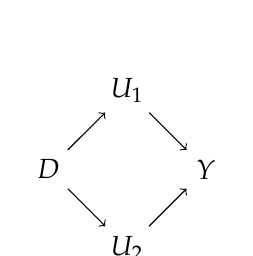
\begin{tikzpicture}
		\node (D) at (0,1) {$D$};
    		\node (UO) at (1,2) {$U_1$};
    		\node (Y) at (2,1) {$Y$};
    		\node (UT) at (1,0) {$U_2$};
    		\path[->] (D) edge (UO);
    		\path[->] (D) edge (UT);
    		\path[->] (UT) edge (Y);
    		\path[->] (UO) edge (Y);
	\end{tikzpicture}
\caption{DAG:faithfulness}
\label{DAG:faithfulness}
\end{figure}
The independence holds if both causal path exactly counteract each other. Needless to say that this kind of occurrence is exceedingly unlikely.
\section{Conditional independence}
Let's revisit the DAG \ref{DAG:Mediator}, we can see that the surgery is correlated to years lived, but the casual path is mediated by the presence of the tumour. A legitimate question one could ask is: if we already have information on B (status of the tumour) does D give us further information? To answer this kind of question we have to control for B, in this case we can restrict the analysis to either one group (B=0, B=1). We represent this restriction by drawing a box around the variable we wish to condition upon. 
\begin{figure}[H]
\centering
\begin{tikzpicture}
		\node (D) at (1,0) {$D$};
    		\node (B)[controlled] (B) at (2,0) {$B$};
    		\node (Y) at (3,0) {$Y$};
    		\path[->] (D) edge (B);
    		\path[->] (B) edge (Y);
\end{tikzpicture}
\end{figure}
We know from assumption \ref{ass:Markov} that any variable in the graph G is independent from any other variable conditioned on its parents, so in this graph we have that $Y \perp\!\!\!\perp D | B$. The result is reasonable  because in this example life expectancy depends directly only on the presence of the tumour, and weather or not the operation was made is entirely irrelevant. 
Conditioning on common effects bears different results, let B the mood of the family (B=0 if sad, B=1 if sad), in this example let's say that the operation has no effect on life expectancy. We can represent this examples with this DAG:
\begin{figure}[H]
\centering
\begin{tikzpicture}
		\node (D) at (1,0) {$D$};
    		\node (B)[controlled] (B) at (2,0) {$B$};
    		\node (Y) at (3,0) {$Y$};
    		\path[->] (D) edge (B);
    		\path[<-] (B) edge (Y);
\end{tikzpicture}
\end{figure}
Let's say that both D and Y have positive effects on B, now if we restrict the analysis on B=0, we will see that patient that are not treated have a low life expectancy, meanwhile in the B=1 we will have patient that are treated and have a higher life expectancy, this is indeed problematic because if we had not controlled for B, D and Y would have been independent. Even though this is just an example, it is proven (citation needed?) that controlling for a collider, or one of it's descendants introduces spurious systematic correlation. Epidemiologist refer to this spurious correlation as \textit{selection bias under the null}. When we condition on a common effect we open the flow of association through the graph.
As we have seen earlier common causes, like DAG \ref{DAG:Common cause}, produce systematic bias that we will refer to as \textit{confounding bias}. Now let B be inflammation status that both causes lower life expectancy (Y) and a higher chance of being operated (D). 
\begin{figure}[H]
	\centering
	\begin{tikzpicture}
		\node (D) at (0,0) {$D$};
    		\node (B)[controlled] at (1,1) {$B$};
    		\node (Y) at (2,0) {$Y$};
    		\path[<-] (D) edge (B);
    		\path[->] (B) edge (Y);
	\end{tikzpicture}
\end{figure}
Let's imagine restricting the analysis to B = 1 (inflammation present), we can clearly see that a lower life expectancy doesn't tell us any new information on the chance of being operated. 
We can also deduce this by applying the Markov assumption that tells us that $D \perp\!\!\!\perp Y|B$, since B is the parent of both Y and D. When we condition on a common cause we close the flow of association through the graph.
% grafico strano 
%\begin{figure}
%	\caption{Graph 1}
%	\large{\begin{tikzpicture}[%
%		->,
%		>=stealth,
%		node distance=1cm,
%		pil/.style={
%			->,
%			thick,
%			shorten =2pt,}
%		]
%		\node (1) {Y};
%		\node[left=of 1] (2) {A};
%		\node[right=of 1] (3) {L};
%		\draw [->] (1.east) -- (3.west);
%		\draw [->] (2) to [out=30, in=150] (3);
%	\end{tikzpicture}}
%\end{figure}
%grafici validi e non validi 
% magari metterli di fianco 
%\begin{figure}[ht]
%  \subcaptionbox{First subfigure}[.22\linewidth]{%
%	\begin{tikzpicture}
%		\node (A) at (0,0) {$A$};
%    		\node (B) at (1,0) {$B$};
%    		\node (C) at (2,0) {$C$};
%    		\path[<-] (A) edge (B);
%    		\path[->] (B) edge (C);
%	\end{tikzpicture}
%  }%
%  \hfill
%  \subcaptionbox{Second subfigure}[.22\linewidth]{%
%	\begin{tikzpicture}
%		\node (A) at (0,0) {$A$};
%    		\node (B) at (1,0) {$B$};
%    		\node (C) at (2,0) {$C$};
%    		\path[<-] (A) edge (B);
%    		\path[->] (B) edge (C);
%	\end{tikzpicture}
%  }
%  \subcaptionbox{First subfigure}[.22\linewidth]{%
%	\begin{tikzpicture}
%		\node (A) at (0,0) {$A$};
%    		\node (B) at (1,0) {$B$};
%    		\node (C) at (2,0) {$C$};
%    		\path[<-] (A) edge (B);
%    		\path[->] (B) edge (C);
%	\end{tikzpicture}
%  }%
%
%\end{figure}

\section{Back door criterion}
\label{sect:backdoor}
If we want to be able to tell weather a casual effect is identifiable we have to satisfy the \textit{backdoor criterium}. We satisfy this criterium if and only if all back-door paths are blocked i.e. if all non direct flow of association are blocked and we don't condition on a descendant of the exposure [citation needed for the last part].
We can define a path to be blocked or open by these graphical rules \citep{hernan2020causal}:
\begin{enumerate}
\item if there are no variables being conditioned on, a path is blocked if and only if there is a collider
\item Any path that contains a non-collider that has been conditioned on is blocked. 
\item A collider that has been conditioned on does not block a path. 
\item A collider that has a descendant that has been conditioned on does not block a path. 
\end{enumerate}
Let's make this rules clearer by applying them to a few examples: 
Ex1. [should I expand every example with a story]
\begin{figure}[H]
\centering
	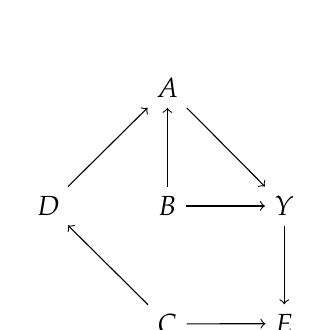
\begin{tikzpicture}
		\node (D) {$D$} ;
		\node (B) [right = of D] {$B$};
    		\node (Y) [right = of B] {$Y$};
    		\node (A) [above = of B] {$A$};
    		\node (C) [below = of B] {$C$};
		\node (E) [below = of Y] {$E$};
		\path[->] (D) edge (A);
    		\path[->] (B) edge (Y);
    		\path[->] (B) edge (A);
		\path[->] (A) edge (Y);
		\path[<-] (D) edge (C);
		\path[->] (C) edge (E);
		\path[->] (Y) edge (E);
	\end{tikzpicture}
\end{figure} 
Let's list all paths from our intervention D to Y : we have  $D \rightarrow A \rightarrow Y$ and $D \rightarrow A \leftarrow B \rightarrow Y $  these two are not back-door paths, so we don't have to control for anything to avoid modifying the main causal path. The only back-door path we need to worry about is $D \leftarrow C \rightarrow E \leftarrow Y $, we see from graphical rule number 1, that a path is closed if there is a collider that in this case is $E$. We can see than that we don't have to control for anything; the causal effect is identifiable. 
Example n.2 
\begin{figure}[H]
\centering
	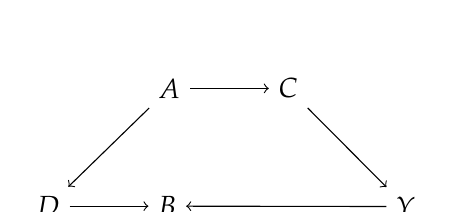
\begin{tikzpicture}
		\node (D) {$D$};
		\node (A) [above right = of D] {$A$};
    		\node (C) [right = of A] {$C$};
    		\node (Y) [below right = of C] {$Y$};
    		\node (B) [right = of D] {$B$};
		\path[<-] (D) edge (A);
    		\path[->] (A) edge (C);
    		\path[->] (C) edge (Y);
		\path[->] (D) edge (B);
		\path[->] (Y) edge (B);
	\end{tikzpicture}
\end{figure} 
Here we have two paths $D \rightarrow B \leftarrow Y $ and a backdoor path witch is $D \leftarrow A \rightarrow C  \rightarrow Y$. We ought not to condition on B because it's a common cause and would introduce spurious correlation; meanwhile we should condition on A since is a common cause of $D$ and $G$. The resulting DAG would be:
\begin{figure}[H]
\centering
	\begin{tikzpicture}
		\node (D) {$D$};
		\node (A)[controlled] [above right = of D] {$A$};
    		\node (C) [right = of A] {$C$};
    		\node (Y) [below right = of C] {$Y$};
    		\node (B) [below = of A] {$B$};
		\path[<-] (D) edge (A);
    		\path[->] (A) edge (C);
    		\path[->] (C) edge (Y);
		\path[->] (D) edge (B);
		\path[->] (Y) edge (B);
	\end{tikzpicture}
\end{figure} 
Once we followed all the rules and no paths the causal effect will be identifiable and any systematic correlation between exposure and outcome can be interpreted as the causal effect $D_i$ has on $Y_i$.

%
%\begin{figure}[H]
%\centering
%	\begin{tikzpicture}
%		\node (D) {$D$} ;
%		\node (Y) [right = of D] {$Y$};
%    		\node (B) [below = of D] {$B$};
%    		\node (A) [right = of B] {$A$};
%		\path[->] (D) edge (Y);
%    		\path[->] (D) edge (B);
%    		\path[->] (B) edge (Y);
%		\path[->] (A) edge (B);
%		\path[->] (A) edge (Y);
%	\end{tikzpicture}
%\end{figure} 
%
%
 
\chapter{Potential outcome model}
\label{chapt:PotentialOM}
The potential outcome model defines the causal effect of an event A as the difference between the two possible states of the world, namely the world where A occurs and the one where A does not occur.
For example, we would like to understand if a medicine can truly improve headaches. Let's formalize the problem by setting X as the set of patient covariates (Age , Gender,... ), D as the treatment regimen (set equal to 1 if the patient takes the medicine and 0 if he takes the placebo), and $Y$ as the number of minutes the headache persists.
Under this model the causal effect of the medicine would be calculated by subtracting $Y_i|D=1$, which we'll call $Y^{1}_i$, and $Y_i|D=0$ which we'll call $Y^{0}_i$. These are the so called "potential outcome" because they are both \textit{a priori} observable, but only one can be observed \textit{a posteriori}. Let's introduce a numerical example of a random trial, where we somehow know both potential outcomes :

\begin{table}[H]
\centering
\begin{tabular}{|c|c|c|c|c|}
\hline
Age & Sex & $Y^{0}_i$ & $Y^{1}_i$ & $\delta_i$ \\ \hline
20 & M & 20 & 21 & -1  \\ \hline
20 & F & 15 & 3 & 12 \\ \hline
20 & M & 8 & 10 & -2 \\ \hline
20 & F & 16 & 15 & 1 \\ \hline
30 & M & 12 & 13 & -1 \\ \hline
30 & F & 8 & 5 & 3 \\ \hline
30 & M & 2 & 11 & -9  \\ \hline
30 & F & 15 & 26 & 11 \\ \hline
\end{tabular}
\caption{Random trial knowing both potential outcomes }
\label{rt_kbpo}
\end{table}

We can observe that $\delta$ isn't always positive, so the medicine didn't universally improve the situation, but it is seemingly clear that it had positive effects, this isn't nearly precise enough so we need to introduce some mathematical definitions :
\paragraph{Parameter definition} \hspace{0pt} \\
\label{parag:param}
\begin{itemize}
\item CATE or Conditional Average Treatment Effect is defined as $E[Y^{1}_i- Y^{0}_i|X] = E[\delta_i|X]$, so $CATE_{(M,20)}=E[\delta_i|X=(M,20)] \approx \frac{18-2}{2}=8$ , we can say that on the medicine caused a reduction on average of 8 minutes between 20 year old males.
\item ATE or Average Treatment Effect is defined as  $E[Y^{1}_i- Y^{0}_i] = E[\delta_i]$, quindi $ATE= E[\delta_i] \approx \frac{18+12-2+18+3-9+11}{8}$.
\item ATT o Average Treatment on the Treated is defined as  $E[Y^{1}_i- Y^{0}_i|D=1] = E[\delta_i|D=1]$ 
\item ATU o Average Treatment on the Untreated is defined as
$E[Y^{1}_i- Y^{0}_i|D=1] = E[\delta_i|D=1]$
\end{itemize}
 

In this example we somehow know both potential outcomes so we can't calculate the last two quantities.
It useful to make a distinction between \textit{factual} and \textit{counter factual} values, the former refers to the state of the world we are currently in and the latter refers to \textit{what would have been} if the treatment were different.
We can better understand the distinction between the two through the switching equation: 
\begin{equation}
Y_i^{obs} = D_i \cdot Y^1_i + (1-D_i) \cdot Y^0_i
\label{eq:switching}
\end{equation}
We can see that $Y^1_i$ is either a \textit{factual} value when $D_i=1$ or \textit{counter factual} when $D_i=0$.
It's obvious that in real setting, we wont ever be able to fill all the data like in table \ref{rt_kbpo}, at least half of the value will be missing and Bayesian methods will help us fill it.
An example of such table could be this:
\begin{table}[H]
\centering
\begin{tabular}{|c|c|c|c|}
\hline
Age & Sex & $Y^{0}_i$ & $Y^{1}_i$ \\ \hline
20 & M & 20 & ?  \\ \hline
20 & F & 15 & ? \\ \hline
20 & M & ? & 10 \\ \hline
20 & F & ? & 15  \\ \hline
30 & M & 12 & ? \\ \hline
30 & F & 8 & ? \\ \hline
30 & M & ? & 11   \\ \hline
30 & F & ? & 26 \\ \hline
\end{tabular}
\caption{Tabella esperimento }
\end{table}
The potential outcome model manages to transform the intractable problem of causation in to a much more manageable problem of \textit{missing data}.

\section{Assumptions and exclusion restriction}
So far we hid a few of the assumption that are necessary for an easier  introduction. 
Let's start with the most important \textit{exclusion restriction} that is  an assumption that rely on external, substantive, information to 

\citep{imbens2015causal}

\subsection{SUTVA}
\begin{ass}
The potential outcome for any unit do not vary with the treatments assigned to other units and, for each unit, there are no different forms or versions of each treatment level, which lead to different potential outcomes.
\label{sutva}
\end{ass}
\citep{imbens2015causal}
\ref{sutva}

\subsection{Ignorability}

"fan li : a tutorial on causal inference"
\subsection{Superpopulation and finite samples}



\section{Studi randomizzati: Ruolo della randomizzazione}
We often hear about double-blind randomized trials, where some of the patients are given the medicine and the other are given a placebo with neither the doctors nor the patients aware of who received what. Such trial can be expressed through a DAG in this way: 
\begin{figure}[H]
\centering
	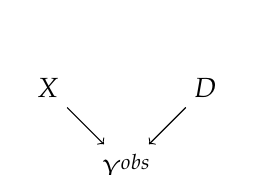
\begin{tikzpicture}
		\node (x) at (0,1) {$X$};
    		%\node (yz) at (0,0) {$Y^{1}$};
    		%\node (yo) at (2,0) {$Y^{0}$};
		\node (y) at (1,0) {$Y^{obs}$};
    		\node (D) at (2,1) {$D$};
    		%\path[->] (x) edge (yz);
    		%\path[->] (x) edge (yo);
    		\path[->] (x) edge (y);
    		%\path[<-] (T) edge (x);
    		\path[->] (D) edge (y);
	\end{tikzpicture}
\caption{Dag per studio randomizzato}
\label{fig:dag_random_EX}
\end{figure}
Why is this kind of trial become the golden standard for causal inference? What can such a trial truly tell us?
Under the potential outcome model this kind of trial imply this independence:
\begin{equation}
D \perp\!\!\!\perp (Y^{0},Y^{1})
\end{equation}
\label{eq:indipendence_r}

This means that the potential outcomes didn't play a role in determining the treatment regime. This \textbf{doesn't} imply that $D \perp\!\!\!\perp Y^{obs}$, in fact is patently false each time a medicine has an effect on patient. By virtue of equation \ref{eq:indipendence_r}, we can state that $E[Y^1_i] = E[Y^{1}_i | D_i = 1]  $ and the same for $E[Y^0_i] = E[Y^{0}_i | D_i = 0] $.
We can than say that:
\begin{align}
ATE &= E[Y^1_i-Y^0_i ] \\ 
 &= E[Y^{1}_i | D_i = 1]- E[Y^{0}_i | D_i = 0]\label{eq:ATE_R} \\
	& =E[Y^{1}_i | D_i = 1]- E[Y^{0}_i | D_i = 1] \label{eq:ATT_R} \\
 &= E[Y^{1}_i | D_i = 0]- E[Y^{0}_i | D_i = 0] \label{eq:ATU_R}
  \end{align}
In the equation \ref{eq:ATE_R} both quantities are \textit{factual}, through the law of large number we can estimate both as means. We will define as SDO the simple difference in means in the observation:
$$SDO := \frac{1}{N_1}\sum_{i:d_i=1}y_i - \frac{1}{N_2}\sum_{i:d_i=0}y_i \overset{\underset{\mathrm{(N_1, N_2) \rightarrow \infty}}{}}{=} ATE$$

We can also conclude from equation \ref{eq:ATT_R} and \ref{eq:ATU_R} that in a randomized trial we have $ATE = ATT = ATU$.
\subsection{Parte empirica}

% crucial to understand the difference bewteen definition and estimation 
\section{Observational studies} % esiste il termine?
Observational studies are much different, researchers gather data that isn't intended to be randomized trials, were the researchers cannot intervene and impose the randomization, for two main reason :
\begin{enumerate}
\item Ethical or practicability concerns  (EX: if we wanted to know whether smoking causes cancer)
\item The events might have already taken place  (EX: if we wanted to study the effect of a certain policy)
\end{enumerate}

The main difference is that $D \not \perp\!\!\!\perp (Y^{0},Y^{1})$, we can represent this too with a DAG:
\begin{figure}[!h]
\centering
	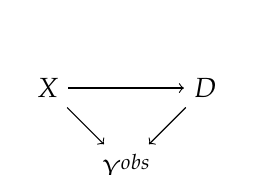
\begin{tikzpicture}
		\node (x) at (0,1) {$X$};
    		%\node (yz) at (0,0) {$Y^{1}$};
    		%\node (yo) at (2,0) {$Y^{0}$};
    		\node (y) at (1,0) {$Y^{obs}$};
    		\node (D) at (2,1) {$D$};
    		%\path[->] (x) edge (yz);
    		%\path[->] (x) edge (yo);
    		\path[->] (x) edge (D);
    		\path[->] (x) edge (y);
    		\path[->] (D) edge (y);
    		%\path[<-] (T) edge (x);
    		%\path[->] (T) edge (y);
	\end{tikzpicture}
\caption{Dag per studio osservazionale}
\label{fig:dag_OBS}
\end{figure}
%\citet{pacesalvan}

%\backmatter

\cleardoublepage
%\addcontentsline{toc}{chapter}{References}

\fancyhf{} % rimuove l'attuale contenuto dell'intestazione
\fancyhead[LE,RO]{\thepage \sffamily}
\fancyhead[LO,RE]{\textit{Bibliografia}}

\bibliographystyle{biblio_style.bst}
\bibliography{biblio} %Bibliography file
\nocite{*} 

\end{document}


